\documentclass[number=03]{assignment}
\title{Computer Architecture - TE2003B}
\chead{Assignment 02}
\rhead{\acs{ISA} and \acs{uA}}
%\date{February - June 2020}

\newif\ifanswers
\answerstrue % comment out to hide answers

\newcommand{\deadline}{23:59 hours on Friday November 26th 2021}
% Begin document
\begin{document}

\setcounter{chapter}{1}
\chapter*{Assignment 02 \\ \acl{ISA} and \acl{uA} design}
\acresetall
% ======================================
% Objective
% ======================================
\section{Objectives}
To understand how the \ac{ISA} influences \ac{uA} design. 

% ======================================
% Deadline
% ======================================
\section{Deadline}
\alertblue{\deadline}.
% ======================================
% Teamwork policy
% ======================================
\section{Teamwork policy}
This is a group assignment. You may work in teams of up to three students.
% % ======================================
% % Pre-requisites
% % ======================================
% \section{Pre-requisites}
% It is assumed that you are familiar with working with \ModelSim and \Quartus. 
% If you require assistance, you can refer to the first assignment tutorial.
% ======================================
% Background
% ======================================
\section{Background}\label{Sec:Background}
Assume that we have designed a \ac{uA} of an \ac{ISA} that can only perform a single addition of two numbers.
The \ac{ISA} specifies the following.
\begin{enumerate}
\item The operands for the addition must be retrieved from a \ac{RF}.  
\item The addition must be done in the form \Rd $\leftarrow$ \Rs{1} + \Rs{2}, where \Rd is the destination register and \Rs{1} and \Rs{2} are the two source registers, respectively.
\item There are only four registers \code{Ri} available, where $i\in[0,3]$
\item Any two registers may be added together.
\item The result may be stored in any register.
\end{enumerate}
So far, we have designed an instruction encoding for this \ac{ISA}, as shown in \tref{Table:basic_encoding}.
% Encoding table
%
  %
  % Figure naive uA
  %
% \begin{figure}[!htb]
%  \centering
%  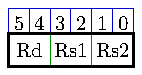
\includegraphics[scale=1.5]{Assignment03_basic_encoding}
%  \caption{Encoding for adding two registers.}
%  \label{Figure:basic_encoding}
%\end{figure} 

\begin{table}[htbp]
    \centering
    \caption{Encoding for adding two registers.}
    \label{Table:basic_encoding}
    \begin{tabular}{|c|c|c|c|c|c|c|}
      \hline
      \textbf{Bit}     & 5 & 4 & 3 & 2 & 1 & 0 \\ \hline
      \textbf{Meaning} & \multicolumn{2}{c|}{Rd} & \multicolumn{2}{c|}{Rs1} & \multicolumn{2}{c|}{Rs2} \\
      \hline
  	\end{tabular}
  \end{table}
  %
  % End Figure naive uA
  %
%
% End Encoding table
%

Note that so far, our \ac{ISA} only performs one type of operation.
As a result of this, we do not require an \codeblue{opcode} field in the encoding of \tref{Table:basic_encoding}.
 
\newpage
%\newline  
Selected expanded examples of the encoding of \tref{Table:basic_encoding} are provided in \tref{Table:naive_instruction_encoding_example}.  
  %
  % Encoding expanded example
  %
  \begin{table}[htbp]
    \centering
    \caption{Selected expanded examples of the instruction encoding for adding two registers.}
    \label{Table:naive_instruction_encoding_example}
    \begin{tabular}{c|c|c}
      \hline
      \textbf{Instruction} & \textbf{Binary Encoding} & \textbf{Hex encoding}\\
      \hline\hline
      \code{\R0 $\leftarrow$ \R0 + \R0} & 00 0000 & \hex{00} \\ \hline
      \code{\R0 $\leftarrow$ \R0 + \R1} & 00 0001 & \hex{01} \\ \hline
      \vdots                            & \vdots & \vdots  \\ \hline
      \code{\R1 $\leftarrow$ \R2 + \R3} & 01 1011 & \hex{1B} \\ \hline
      \vdots                            & \vdots & \vdots  \\ \hline
      \code{\R2 $\leftarrow$ \R3 + \R0} & 10 1100 & \hex{2C} \\ \hline
      \vdots                            & \vdots & \vdots  \\ \hline
      \code{\R3 $\leftarrow$ \R3 + \R3} & 11 1111 & \hex{3F} \\ \hline
  	\end{tabular}
  \end{table}
  %
  % End Encoding expanded example
  %
  
The encoding from \tref{Table:basic_encoding} and \tref{Table:naive_instruction_encoding_example} has been implemented using the \uA shown in  \fref{Figure:NaiveuA}. 
Here, signals such as \code{clock} and \code{reset}, as well as status flags such as \code{c}, \code{v}, \code{n} and \code{v} have been omitted for simplicity. 
Moreover, $n$ simply represents a data bus of $n$-bits, which is assumed to be the number of data bits in the architecture.
  %
  % Figure naive uA
  %
 \begin{figure}[!htb]
  \centering
  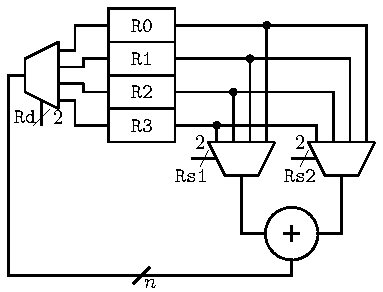
\includegraphics[width=0.57\linewidth]{ISA_naive_uA_example}
  \caption{\uA for adding two registers.}
  \label{Figure:NaiveuA}
\end{figure} 
  %
  % End Figure naive uA
  %

% ======================================
% ISA and uA
% ====================================== 
\newpage
\section{\ac{ISA} and \ac{uA} improvement}\label{Sec:ISA_Improvement}
In this assignment, you are required to improve both the \ac{ISA} and \ac{uA} from \sref{Sec:Background} by including another addressing mode and by performing additional arithmetic operations.
More specifically, the improved \ac{ISA} must be able to perform additions, subtractions, multiplications and divisions by reading/storing data from/to both the \ac{RF} and \ac{DM}.
For this part of the assignment, you may assume the following.
\begin{enumerate} 
  \item There are only eight registers \code{Ri} available, where $i\in[0,7]$.\label{item:1} 
  \item There are only eight memory locations \code{Mem[i]} available, where $i\in[0,7]$.\label{item:2}
  \item Any valid combination of \code{Ri} and \code{Mem[i]} is possible.\label{item:3}
  More specifically, each of the four arithmetic operations may be performed between:
  \begin{enumerate}
  \item Any two registers.
  \item Any register and any memory location.
  \item Any two memory locations.
  \end{enumerate}  
   \item Your design should be able to store the arithmetic result in any register or in any memory location.\label{item:4}
   \item Memory locations may only be accessed in the form \code{Mem[i]}, $i \in [0,7]$, \ie, \code{Mem[0], Mem[1], ..., Mem[6], Mem[7]}.\label{item:5}
\end{enumerate}

Your task is to improve both the \ac{ISA} and \ac{uA} from \sref{Sec:Background} in order to support the specifications described in \cref{item:1,item:2,item:3,item:4,item:5} of this section.
You should start by modifying the instruction encoding of \tref{Table:basic_encoding} and \tref{Table:naive_instruction_encoding_example} in order to include the new arithmetic operations and the new addressing mode.
Following this, you should be able to draw a schematic diagram of a \ac{uA} similar to \fref{Figure:NaiveuA} that supports your improved \ac{ISA}. 
%
\section{Deliverables and Submission instructions}\label{Sec:Deliverables}
Prepare a \code{pdf} file answering the following questions.
\begin{enumerate}
%\item \marking{5} What type of instruction encoding is the encoding of~\tref{Table:basic_encoding} and \tref{Table:naive_instruction_encoding_example}?
%\item \marking{5} What type(s) of memory addressing does the encoding from \tref{Table:basic_encoding} and \tref{Table:naive_instruction_encoding_example} support?
\item \marking{10} Draw a table similar to \tref{Table:basic_encoding} with your selected encoding for supporting \ac{DM} access and all four arithmetic operations.
Your encoding \alertred{must} explicitly name the new fields you have added, for example, \codeblue{opcode} and \codeblue{addressing\_mode}.\label{question:encoding}
\item \marking{10} Draw a table similar to \tref{Table:naive_instruction_encoding_example}, showing \alertblue{a few representative} expanded examples of your encoding for the improved \ac{ISA}.\label{question:encoding_example}
\item \marking{65} Draw a schematic diagram of a \uA that supports your improved encoding from questions \ref{question:encoding} and \ref{question:encoding_example} in this section.
Make sure to label all signals, especially \ac{MUX} selector signals. 
However, in order to improve the readability of your schematic, do not include signals such as \code{clock}, \code{reset}, and the \ac{ALU} status flags.
Similarly, assume that the result of all arithmetic operations may be correctly represented using $n$-bits.
Moreover, you may further simplify your schematic by using an \ac{ALU} block consisting of two operand inputs, one operation selector input, and one result output.
%\item \marking{10} What type of instruction encoding is your improved design?
%\item \marking{10} What type(s) of memory addressing does your improved design support?
\item \marking{15} In 5 sentences or less, explain how your \uA works for your selected encoding.
\end{enumerate} 

\alertblue{IMPORTANT!} 

Since this assignment involves \ac{uA} design, there may be \alertviolet{multiple} correct answers.

Submit your assignment through Canvas \alertred{no later} than \deadline. 
\\

Please send any questions to \href{mailto:isaac.perez.andrade@tec.mx}{isaac.perez.andrade@tec.mx}.
\end{document}
s